

%%% BEGIN CHAPTER 2 MICROARRAY %%%

%% Paper title page %%
\chapter[PLZF expression maps the early stages of ILC1 lineage \\ development]{PLZF expression maps the early stages of ILC1 lineage development}

% authors
Michael G. Constantinides\U{a}, Herman Gudjonson\U{b}, Benjamin D. McDonald\U{a}, Isabel E. Ishizuka\U{a}, Philip A. Verhoef\U{a}, Aaron R. Dinner\U{a,b,c}, and Albert Bendelac\U{a,1}
\\ \\
\U{a}Committee on Immunology,\\
\U{b}Institute for Biophysical Dynamics, and \\
\U{c}Department of Chemistry, University of Chicago, Chicago, IL 60637 
\\
\U{1}To whom correspondence should be addressed. Email\: abendela@bsd.uchicago.edu
\\ \\
Author contributions: M.G.C. and A.B. designed research; M.G.C., H.G., B.D.M., I.E.I., and P.A.V. performed research; M.G.C., H.G., A.R.D., and A.B. analyzed data; M.G.C. and A.B. wrote the paper; and H.G. performed bioinformatics analysis.
\\ \\
Published in PNAS March 11, 2015; doi:10.1073/pnas.1423244112

\newpage
\section{SIGNIFICANCE}
Diverse populations of group 1 innate lymphocytes, which exert critical early cytolytic functions against virally infected cells, have recently been discovered, raising issues of lineage relationships. We used expression of the transcription factor promyelocytic leukaemia zinc finger (PLZF) to identify the developmental intermediates of innate lymphoid cells type 1 (ILC1s), a subset of innate lymphoid cells that are particularly abundant in the liver, and demonstrated that this lineage arises from a distinct precursor, but that its development partially overlaps with established classical NK stages. Using microarray analysis, we defined a set of PLZF-dependent genes that may contribute to lineage divergence between ILC1s and classical NK cells.

\section{ABSTRACT}

Among the variety of tissue-resident NK-like populations recently distinguished from recirculating classical NK (cNK) cells, liver innate lymphoid cells (ILC) type 1 (ILC1s) have been shown to represent a distinct lineage that originates from a novel promyelocytic leukaemia zinc finger (PLZF)-expressing ILC precursor (ILCP) strictly committed to the ILC1, ILC2, and ILC3 lineages. Here, using PLZF-reporter mice and cell transfer assays, we studied the developmental progression of ILC1s and demonstrated substantial overlap with stages previously ascribed to the cNK lineage, including pre–pro-NK, pre-NK precursor (pre-NKP), refined NKP (rNKP), and immature NK (iNK). Although they originated from different precursors, the ILC1 and cNK lineages followed a parallel progression at early stages and diverged later at the iNK stage, with a striking predominance of ILC1s over cNKs early in ontogeny. Although a limited set of ILC1 genes depended on PLZF for expression, characteristically including \textit{Il7r}, most of these genes were also differentially expressed between ILC1s and cNKs, indicating that PLZF together with other, yet to be defined, factors contribute to the divergence between these lineages.

\section{INTRODUCTION}

NK cells represent the longest and best studied population of innate lymphocytes, whose roles in host defense against infections, particularly viral infection by cytomegalovirus, and in tumor or transplant rejection have been extensively characterized \cite{sun2009,yokoyama2004,vivier2011}. The core NK program is based on a panoply of NK-lineage receptors specific for MHC and MHC-like ligands that are induced by stress and infection to trigger perforin- and granzyme-mediated cytolysis of target cells and secretion of type 1 cytokines. This program is controlled in part by the transcription factor T-bet, the related factor eomesodermin, and the cytokine IL-15.

NK cells were long considered to be a single lineage phenotypically characterized by the surface \CDte\UM NK1.1\UP DX5\UP{} profile of its mature product. However, several recent studies have revealed the existence of distinct subpopulations of NK-like cells that, unlike the recirculating classical NK (cNK) cells found in spleen, blood, and lymph nodes, exhibited the unusual property of long-term residence in particular tissues, including liver, intestinal epithelium, uterus, skin, and salivary glands \cite{sojka2014,yokoyama2013,peng2013,cortez2014, fuchs2013,sojka2014review}. For example, in parabiotic pairs of CD45\UM{} congenic mice, a fraction of \CDte\UM NK1.1\UP liver cells were found to be tissue-resident rather than recirculating cells (6). The resident cells were further distinguished from cNK cells by the expression of the TNF family member TNFSF10 (TRAIL), the presence of high levels of integrin $\alpha$1 chain (CD49a), the absence of integrin $\alpha$2 (CD49b, stained by the DX5 antibody), and the expression of CD160, a receptor for epithelium-expressed HVEM \cite{sojka2014,peng2013,fuchs2013,klose2014}. Whereas, like cNKs, the liver-resident cells expressed T-bet and were endowed with cytolytic and type 1 cytokine secretion properties, they characteristically lacked eomesodermin and expressed some level of surface IL7R$\alpha$ chain \cite{sojka2014,klose2014,daussy2014}. Although their DX5\UM phenotype initially suggested they were immature NK cells \cite{takeda2005,gordon2012,vosshenrich2013}, further studies based on fate mapping and cell transfers into \Ragrg hosts established that they represented a different lineage, originating from a small subset of lineage (Lin)\UM IL7R$\alpha$\UP \ab\U{high} Id2\U{high} bone marrow or fetal liver cells that transiently but characteristically expressed high amounts of the transcription factor promyelocytic leukaemia zinc finger (PLZF) \cite{klose2014,constantinides2014}. This PLZF-expressing precursor was termed the ILC precursor (ILCP) because it also generated ILC2s and ILC3s, but, importantly, generated only few cNK-like cells and did not give rise to LTis, B, or T cells \cite{constantinides2014}. Consistent with these findings, most innate lymphoid cells type 1 (ILC1s) were fate-mapped by PLZF, whereas, in contrast, cNKs were generally not fate-mapped, with the notable exception of a small fraction of cNKs, which perhaps originated from ILCPs that retained some cNK potential or, alternatively, were derived from rare cNK precursors that might express low level of PLZF. Thus, these findings altogether supported the notion that ILC1s and cNKs primarily originated from different precursors. Furthermore, although there remain a few discrepancies in the description of these cells by different groups, in particular regarding the degree of requirement for the transcription factor Nfil3 \cite{sojka2014,yu2014}, it seems clear that the liver-resident NK cells described by Yokoyama and coworkers are largely identical to liver ILC1s \cite{sojka2014}.

The early stages of NK cell development have long been elusive. A \CDte\UM CD122 (IL2R$\beta$)\UP NK1.1\UM{} NK precursor (NKP) subset was first identified based on its ability to generate NK1.1\UP cells upon single cell culture in vitro, albeit with a relatively low clonal frequency of $\sim$1 in 12 \cite{kim2002,rosmaraki2001}. More recent studies, however, have refined the phenotype of these precursors based on the coexpression of CD122 with CD127 (IL7R$\alpha$), CD244, and CD27, identifying a refined NKP (rNKP) as well as an earlier, so-called pre-NKP stage, with a similar phenotype, except for low or absent CD122 \cite{fathman2011}. At the single cell level, both of these populations could generate \CDte\UM NK1.1\UP{} clones at a high frequency of $\sim$1 in 2 in culture with OP9 stromal cells and a mixture of the cytokines SCF, Flt3L, IL-7, and IL-15. In addition, after in vivo transfer into \Ragrg hosts, both populations generated exclusively \CDte\UM NK1.1\UP{} cells in the spleen and liver. Another study used an Id2-GFP reporter strain to identify a population of Lin\UM Id2\U{high} Sca1\UP CD117 (cKit)\U{int/--} CD135 (Flt3)\UM IL7R$\alpha$\UP{} cells, termed pre–pro-NKs \cite{carotta2011}, that generated \CDte\UM NK1.1\UP cells at a frequency of $\sim$1 in 2 upon single-cell culture in vitro with OP9 cells and a mixture of IL-7 and IL-15.

In this study, we used PLZF-IRES-GFPCre reporter mice and cell transfers to examine whether some of these early stages of development might be intermixed with, or reassigned to, ILC1s. We demonstrated considerable heterogeneity, with precursors to ILC1s but also ILC2s and ILC3s present in various proportions at different stages. Furthermore, by transcriptional analysis of PLZF-deficient ILC1s compared with WT ILC1s and cNKs, we identified a PLZF-dependent contribution to the genetic program that differentiates ILC1s from cNKs, which included the characteristic expression of the IL7R$\alpha$ chain. The results help redefine and clarify the early stages of ILC and cNK development and the contribution of PLZF to the divergence of these lineages.

\section{RESULTS}

\subsection{Early NK1.1\UM{} Stages of Development}

We used PLZF-IRES-GFPCre mice to report and fate-map PLZF expression in lymphoid compartments. We previously established that GFP faithfully reported PLZF expression in the hematopoietic compartment, with high levels of expression in ILCP and in NKT cells, but not in other lymphoid subsets \cite{constantinides2014}. However, in fate-mapping experiments based on the ROSA26-fl-STOP-fl-YFP allele, we reported that, whereas a majority of mature ILCs and NKT cells were YFP\UP, as expected, $\sim$30\% of other hematopoietic cells were also YFP\UP, including T, B, myeloid cells, and early hematopoietic cell precursors such as early HSC, LMPP, and CLP cells. This indiscriminate background mapping occurred before hematopoiesis, likely in early embryonic stem cells, because it was readily abrogated in radiation chimeras reconstituted with sorted YFP-negative Lin\UM Sca1\UP cKit\UP (LSK) precursors extracted from PLZF-IRES-GFPCre\UP ROSA26-fl-STOP-fl-YFP mice \cite{constantinides2014}. In the experiments reported below, we used these chimeras, termed YFP-negative chimeras, to faithfully fate-map PLZF expression in the hematopoietic system.

To precisely track the expression of PLZF side by side with fate-mapping at different stages of lymphoid development, we compared GFP expression in straight PLZF-IRES-GFPCre\UP mice with YFP expression in YFP-negative chimeras (Fig. \ref{fig:chap2_F1}). We zoomed in on the pre-NKP and rNKP stages, identified by their Lin\UM IL7R$\alpha$\UP CD27\UP CD244\UP CD117 (cKit)\U{int/low} Flt3\UM{} profile, with the pre-NKP expressing weak or absent CD122 (IL2R$\beta$), and the rNKP expressing high CD122 \cite{fathman2011} as gated in Fig. \ref{fig:chap2_F1}A. Both pre-NKPs and rNKPs were previously shown to selectively reconstitute \CDte\UM NKp46\UP NK1.1\UP Ly49D\UP Ly49H\UP cNK cells in the spleen and liver of \Ragrg mice after in vivo transfer, but a detailed analysis of markers that can identify ILC1s, such as CD49a, DX5, TRAIL, CD127 (IL7R$\alpha$), or eomesodermin, was not reported \cite{fathman2011}. Whereas CLPs failed to express either GFP or YFP, as expected, we found that nearly half of pre-NKPs expressed high amounts of GFP (Fig. \ref{fig:chap2_F1}A), a property previously shown to be restricted to the ILCP \cite{constantinides2014}. Furthermore, at the subsequent rNKP stage, the expression of GFP was down-modulated, both in frequency and in intensity, whereas YFP fate-mapping increased from 15 to 36\% on average (Fig. \ref{fig:chap2_F1}A). These findings suggested that cells with the “pre-NKP” phenotype in fact included a large fraction of PLZF-expressing ILCPs, which subsequently down-regulated PLZF and began to exhibit fate-mapping as they progressed into what was previously described as the “rNKP” stage.

%% Chapter 2 Figure 1 NKP Populations %%
\begin{figure}[p]
\begin{center}
	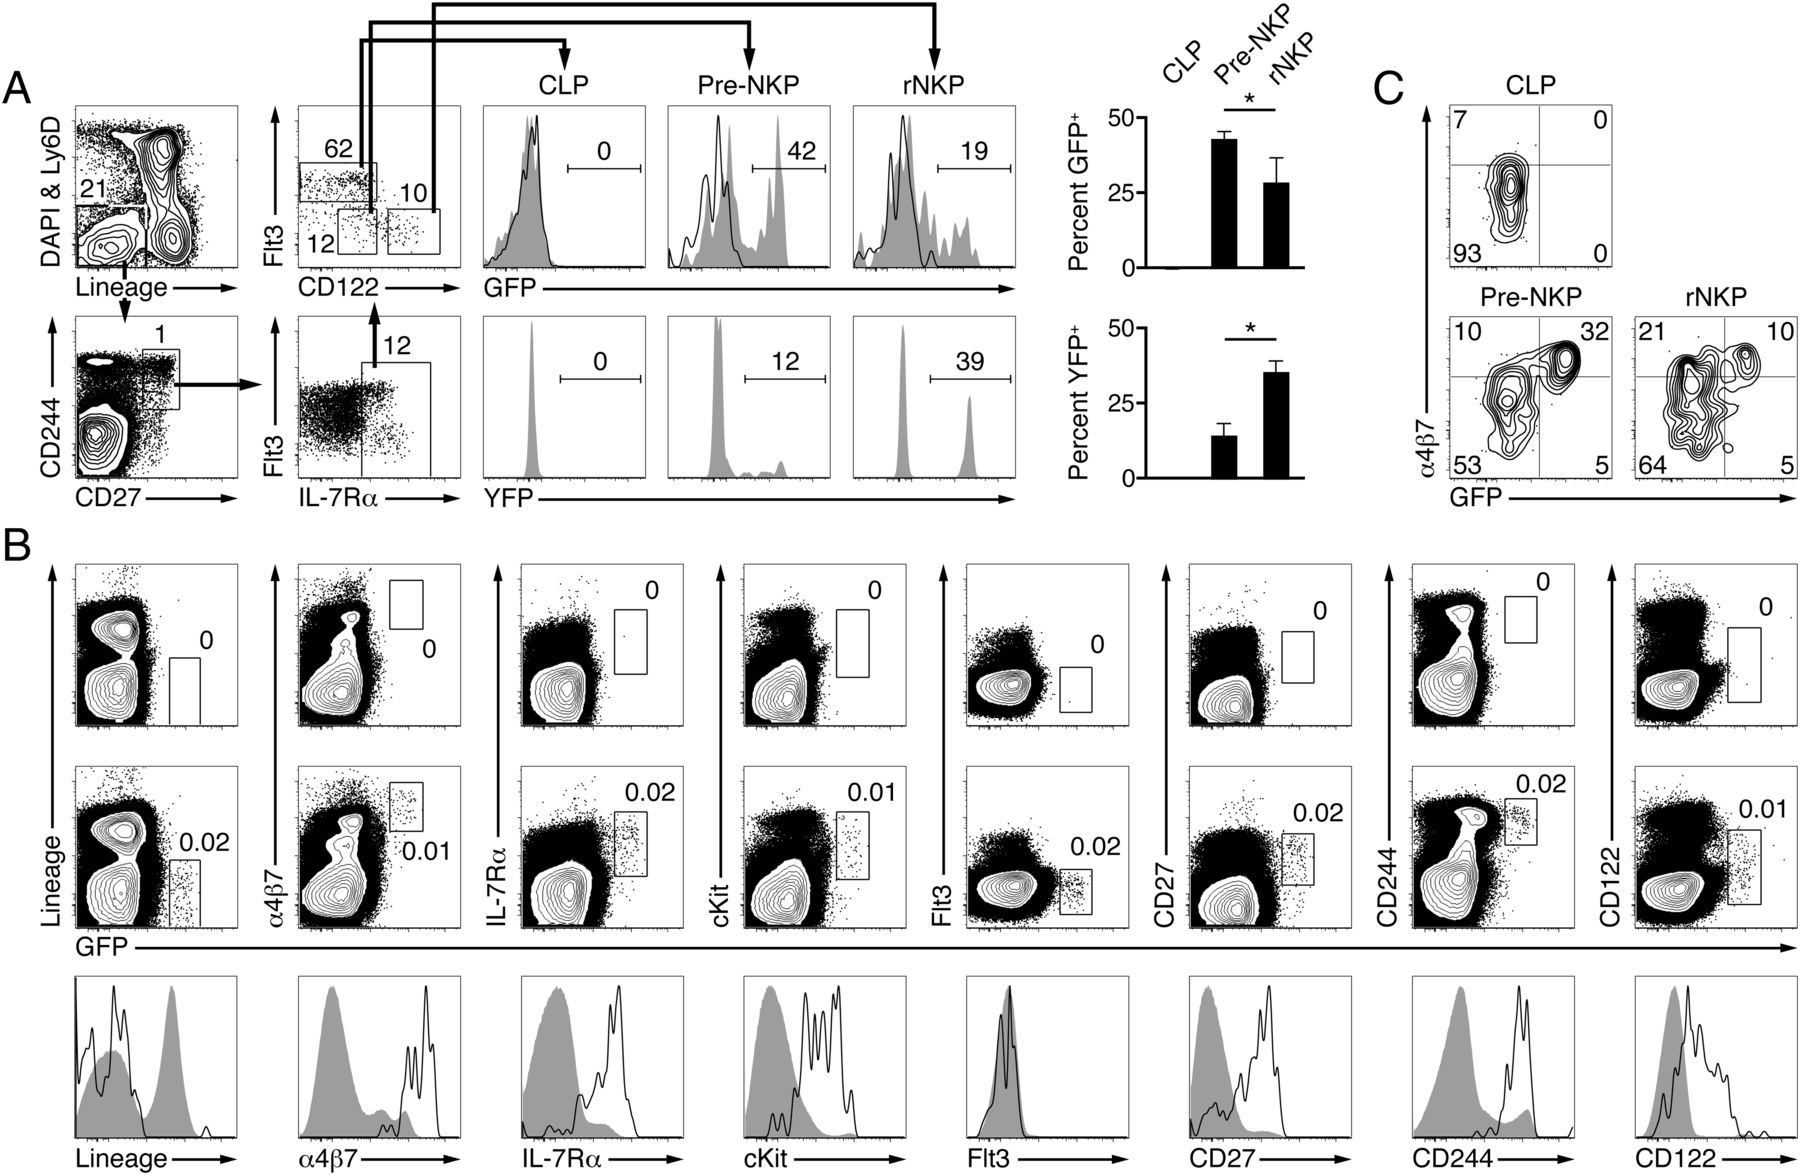
\includegraphics[width=\textwidth]{figures/chapter2/F1}
\end{center}
	\caption{Pre-NKPs and rNKPs are heterogeneous populations.} 
	(A) Gating strategy for CLPs (CD122\UM Flt3\UP), pre-NKPs (CD122\UM Flt3\UM), and rNKPs (CD122\UP Flt3\UM) among Lin\UM Ly6D\UM CD27\UP CD244\UP IL-7R$\alpha$\UP{} bone marrow cells (left four dot plots). Histograms show expression of GFP (reporting PLZF; Top) by the indicated cell types from PLZF\U{GFPcre+/+} (filled gray) and wild-type (open) mice and YFP (reporting fate-mapping by PLZF; Bottom) by the same cell types in YFP-negative chimeras (radiation chimeras reconstituted with YFP\UM Lin\UM Sca-1\UP cKit\UP (LSK) bone marrow cells from PLZF\U{GFPcre+/--} ROSA26-YFP mice). Bar graphs show summary of results (mean $\pm$ SEM). (B) FACS analysis of Ly6D\UM bone marrow cells from adult WT (Top) and PLZF\U{GFPcre+/+} (Middle) mice. Bottom depicts the same results in histogram form with GFP\U{high} (open) and GFP\UM (filled gray) Ly6D\UM bone marrow cells from adult PLZF\U{GFPcre+/+} animals. (C) Expression of GFP and \ab{} by the indicated cell types from PLZF\U{GFPcre+/+} mice. Representative of 3–8 mice analyzed in three or more independent experiments. *$P < 0.05$.
	\label{fig:chap2_F1}
\end{figure}

We therefore extended the comparison between the GFP\U{high} fraction of pre-NKPs and the previously defined ILCPs. Gating on GFP\U{high} cells in the entire bone marrow compartment, we found that these cells not only uniformly expressed the Lin\UM \ab\U{high} CD127 (IL7R$\alpha$)\U{high} CD117 (c-Kit)\UP profile, as previously described for ILCPs, but also were negative for CD135 (Flt3) and positive for CD27 and CD244 (Fig. \ref{fig:chap2_F1}B), the key markers of pre-NKPs \cite{fathman2011}. In contrast, the GFP-negative fraction of pre-NKPs lacked \ab{} expression (Fig. \ref{fig:chap2_F1}C). Because the transition between pre-NKPs and rNKPs is marked by the up-regulation of CD122, we reexamined CD122 expression with a bright antibody-biotin and streptavidin-phycoerythrin combination to detect low quantities of this protein on the cell surface. Indeed, we found that ILCPs expressed variable amounts of surface CD122 that ranged from negative to intermediate and, thus, might include cells already committing to the ILC1 sublineage (Fig. \ref{fig:chap2_F1}B, \textit{Far Right}).

Thus, we conclude that the previously described pre-NKP population is composed of a mixture of ILCPs (precursors to ILC1s, ILC2s, and ILC3s) and cNK precursors. These two fractions can be distinguished by their differential pattern of expression of PLZF and \ab. The distinct progenies of these two fractions can be inferred from transfer experiments showing that the unfractionated pre-NKPs generated classical NK cells in the spleen \cite{fathman2011}, whereas the PLZF\UP \ab\UP (ILCP) fraction did not \cite{constantinides2014}. In retrospect, the failure to observe significant NK1.1\UM progeny (i.e., ILC2 and ILC3) after transfer of pre-NKPs into \Ragrg hosts in the study by Fathman et al. \cite{fathman2011}, is consistent with their focus on spleen and liver, whereas ILC2s and ILC3s predominate in the intestinal lamina propria.

We also examined the Lin\UM Sca1\UP CD117 (cKit)\U{int/--} CD135 (Flt3)\UM IL7R$\alpha$\UP cell, which was proposed to be an early NK precursor, termed pre–pro-NK \cite{carotta2011}. Strikingly, we found uniform but low expression of GFP contrasting with a high frequency of YFP fate-mapping, suggesting that a large fraction of these cells had, in fact, originated from ILCPs and down-regulated PLZF (Fig. \ref{fig:chap2_S1}). Because the majority of these cells also expressed CD25, ICOS, and T1/ST2, the combination of which is highly characteristic of ILC2s, we concluded that they mostly represented late developmental intermediates of ILC2s termed immature ILC2s (iILC2 or LSIG), rather than cNK precursors, consistent with their reported Id2high profile \cite{hoyler2012}. Indeed, cell transfers into \Ragrg hosts have demonstrated that this precursor population exclusively generates mature ILC2 in vivo \cite{hoyler2012}.

\subsection{Immature NKs}

We next examined the so-called immature NK (iNK) cells, which are defined by expression of NKp46 and NK1.1, but not DX5. Although these cells were previously considered to be developmental intermediates of the cNK lineage before acquisition of DX5 \cite{yokoyama2004}, recent reports have emphasized that a fraction of iNKs expressed a phenotype similar to that of mature ILC1s, including expression of IL7R$\alpha$ and CD49a, but neither CD49b (DX5) nor eomesodermin \cite{sojka2014,klose2014,diefenbach2014}. In one study, transfer of eomesodermin-negative iNKs into \Ragrg hosts reconstituted liver ILC1s but not cNKs \cite{klose2014}. We found that nearly 80\% of iNKs, defined by their \CDte\UM CD122\UP NKp46\UP NK1.1\UP DX5\UM{} profile, were YFP\UP, but these cells did not express GFP, suggesting that a large proportion had originated from ILC1 rather than from cNK precursors (Fig. \ref{fig:chap2_F2}A). We further showed that the PLZF fate-mapped iNKs (isolated from YFP-negative chimeras) gave rise exclusively to CD49a\UP DX5\UM (ILC1s) but not to CD49a\UM DX5\UP (cNKs) liver cells after transfer into \Ragrg recipients (Fig. \ref{fig:chap2_F2}B). In contrast, CD45-congenic CLPs (coinjected with the YFP\UP iNKs) generated both cNKs and ILC1s in the liver (Fig. \ref{fig:chap2_F2}B). We also purified bone marrow \CDte\UM NKp46\UP NK1.1\UP DX5\UM{} iNKs, irrespective of their PLZF fate-mapping, and transferred them into \Ragrg hosts, to test whether they contained cNK precursors. Although these cells generated a majority of ILC1s, consistent with the predominance of ILC1 precursors, we also observed a substantial fraction of cNKs (Fig. \ref{fig:chap2_F2}B). Thus, \CDte\UM NKp46\UP NK1.1\UP DX5\UM{} bone marrow cells, previously termed iNKs, are a mixture of both ILC1 and cNK lineage cells, with a strong predominance of ILC1s. Upon stimulation with ionomycin and PMA, the bone marrow \CDte\UM NKp46\UP NK1.1\UP DX5\UM cells produced significantly less IFN-$\gamma$ than their liver counterpart, further supporting the notion that they represented immature ILC1s (iILC1s) (Fig. \ref{fig:chap2_F2}C).

%% Chapter 2 Figure 2 ILC1 and cNK precursors %%
\begin{figure}[p]
\begin{center}
	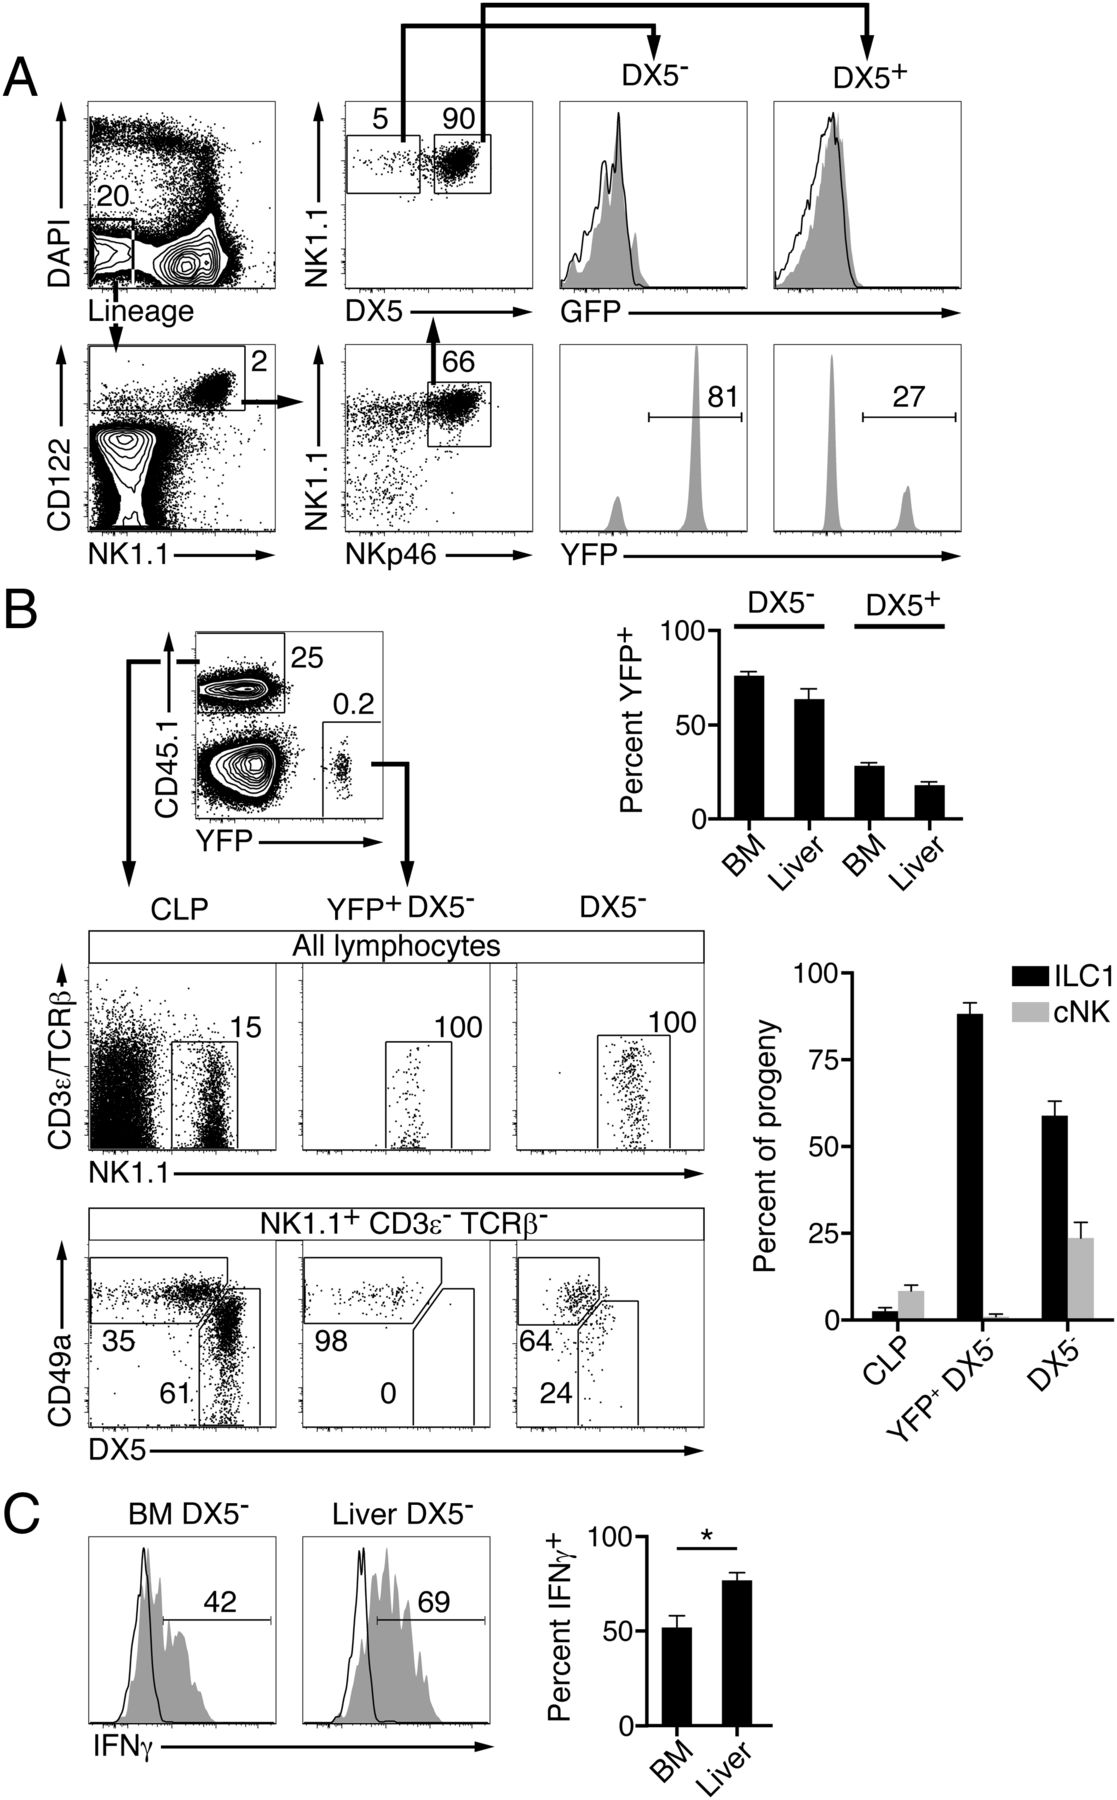
\includegraphics[width=0.4\textwidth]{figures/chapter2/F2}
\end{center}
	\caption{A majority of bone marrow NK1.1\UP DX5\UM “immature NKs” are ILC1 rather than cNK precursors.} 
	(A) Gating strategy for DX5\UM (NK1.1\UP DX5\UM) and DX5\UP (NK1.1\UP DX5\UP) populations among Lin\UM CD122\UP NKp46\UP{} bone marrow cells (left four dot plots). Histograms show expression of GFP (reporting PLZF; Top) by the DX5\UM{} and DX5\UP{} populations from PLZF\U{GFPcre+/+} (filled gray) and WT (open) mice and YFP expression (reporting PLZF fate-mapping; Bottom). Bar graphs show summary of results (mean $\pm$ SEM) for bone marrow DX5\UM{} and DX5\UP{} cells (as gated) and for liver DX5\UM (\CDte\UM TCR$\beta$\UM NK1.1\UP DX5\UM) and DX5\UP (\CDte\UM TCR$\beta$\UM NK1.1\UP DX5\UP) populations. Data representative of 3–5 mice analyzed in three independent experiments. (B) CD45.2 \Ragrg mice were injected with a mixture of 750 CD45.1 CLPs + 1,500 YFP\UP Lin\UM CD122\UP NKp46\UP NK1.1\UP DX5\UM bone marrow cells from YFP\UM chimeras or with 1,500 CD45.1 Lin\UM CD122\UP NKp46\UP NK1.1\UP DX5\UM bone marrow cells alone, as indicated. The progeny of these populations within the liver was analyzed 3–4 wk later by FACS. Bar graphs show summary of results (mean $\pm$ SEM). Representative of 3–5 chimeras analyzed in two independent experiments. (C) The Lin\UM CD122\UP NKp46\UP NK1.1\UP DX5\UM{} bone marrow (BM DX5\UM) and \CDte\UM TCR$\beta$\UM NK1.1\UP DX5\UM{} liver (liver DX5\UM) populations were sorted from WT mice and stimulated with PMA (20 ng/mL) and ionomycin (5 $\mu$g/mL) for 4 h in the presence of 1x GolgiStop, and IFN-$\gamma$ production was analyzed by intracellular FACS staining (filled gray). Control histograms (open) are from unstimulated cells. Results from three independent experiments summarized in the bar graph (mean $\pm$ SEM). *$P < 0.05$.
	\label{fig:chap2_F2}
\end{figure}

Altogether, our analysis of the developmental stages of ILC1s and cNKs suggests a new model whereby these lineages originate from distinct precursors, distinguished by the expression of PLZF and \ab, before undergoing a parallel sequence of progressive steps encompassing previously described populations and diverging between iNKs and iILC1s as proposed in Fig. \ref{fig:chap2_S2}.

\subsection{Predominance of ILC1s Early in Ontogeny}

Tissue-resident ILC1s are reminiscent of the early waves of tissue-resident \gdT cells that populate tissues such as skin, uterus, intestine, liver, and lung in the newborn (23). These tissue-resident \gdT cells express semiinvariant TCRs and are thought to represent a first line of defense in the perinatal period, before the generation of their blood recirculating counterparts, which have a more diverse repertoire. Indeed, we found that a great majority of \CDte\UM NK1.1\UP{} cells in both embryonic day (E)16 fetal liver and in 1-wk-old liver were YFP\UP fate-mapped, expressed CD49a and TRAIL, and lacked eomesodermin, whereas CD49a\UM TRAIL\UM eomesodermin\UP{} cNK cells appeared later in ontogeny between weeks 1 and 3, and were characterized by lower YFP fate-mapping (Fig. \ref{fig:chap2_F3}). Note that to study fetal and newborn hematopoiesis, these experiments used the straight PLZF-IRES-GFPCre crossed to ROSA-fl-STOP-fl-YFP mice, rather than the YFP-negative adult bone marrow chimeras. This experimental necessity explains in part the higher frequency of YFP labeling in cNKs, due to background labeling before the hematopoietic stem cell stage. Surprisingly, liver ILC1s tended to coexpress DX5 in fetal life, but not after birth, emphasizing that DX5 expression may not always be a reliable marker of cNKs. Altogether, these results therefore demonstrate that ILC1s strongly predominate over cNK cells in perinatal life, whereas cNK cells achieve greater frequency in adults.

%% Chapter 2 Figure 3 fetal ILC1 and cNK %%
\begin{figure}[p]
\begin{center}
	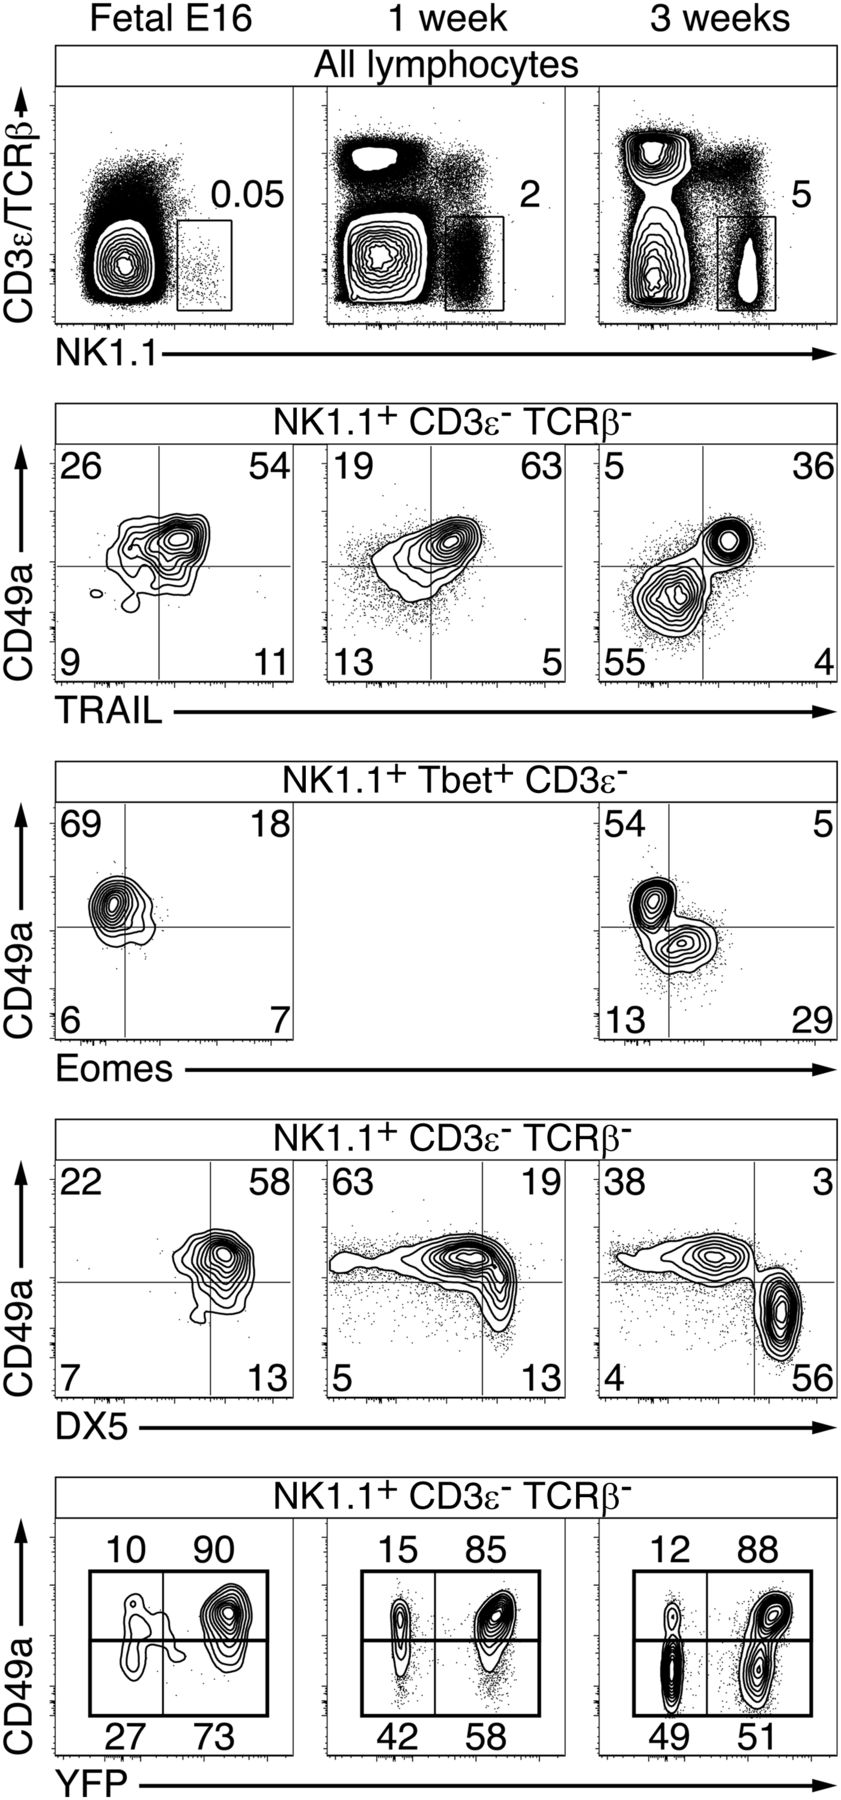
\includegraphics[height=0.5\textheight]{figures/chapter2/F3}
\end{center}
	\caption{Predominance of ILC1s over cNKs in the fetal and newborn liver.} 
	 FACS analysis of hepatic lymphocytes isolated from WT or PLZF\U{GFPcre+/--} ROSA26-YFP mice at E16 or at 1 and 3 wk after birth, as indicated. At Bottom, dot plots are divided into CD49a\UP{} and CD49a\UM{} fractions and the numbers indicate the percentages of YFP\UP{} and YFP\UM{} cells within each of these gates. All dot plots, except on the third row, are obtained from the same samples. Representative of 4–5 mice for each time point, analyzed in two independent experiments.
	\label{fig:chap2_F3}
\end{figure}

Impact of PLZF on ILC1 Development and Maturation. We previously showed that PLZF-deficient ILC1s were decreased fourfold compared with their wild-type counterparts in the liver of competitive bone marrow chimeras \cite{constantinides2014}. By microarray analysis, we found that ILC1s isolated from the liver of PLZF-deficient mice exhibited a limited set of changes compared with those of wild-type littermates, because only 229 genes had altered expression by more than 1.4-fold (Fig. \ref{fig:chap2_F4}A). In contrast, and similar to a recent study \cite{peng2013}, $>$2,000 genes exhibited differential expression between liver cNK cells and ILC1s, indicating that, as expected, the differences between cNKs and ILC1s do not solely depend on PLZF. Strikingly, however, 59\% of the PLZF-dependent genes in ILC1s were also differentially expressed between ILC1s and cNKs, a highly significant overlap ($P = 2.7 \times 10^{−93}$ by hypergeometric test). Because ILC1s and cNKs differ by their history of PLZF expression, these differentially expressed genes may be involved in the divergence between these two lineages. For example, PLZF-deficient ILC1s showed decreased expression of CD127 (IL7R$\alpha$), both at the mRNA level by microarray analysis and at the protein level by flow cytometry (Fig. \ref{fig:chap2_F4} B and C). IL7R$\alpha$ is expressed in the hematopoietic precursors to both ILC1s and cNKs, but its expression is characteristically maintained only in mature ILC1s \cite{diefenbach2014}. Although the role of IL7R$\alpha$ in ILC1 biology is not fully understood, because mature ILC1s seem mostly dependent on IL15 for their maintenance \cite{sojka2014}, it may be important for optimal survival during a developmental window, before expression of the IL15 receptor. Thus, the conspicuous defect in IL7R$\alpha$ expression in PLZF-deficient ILC1s might contribute in part to their decreased frequency. Other ILC1 genes that depended on PLZF and were not expressed by cNKs included \textit{Mmp9}, \textit{Klrb1b}, \textit{Klrk1}, and \textit{Tnfrsf25}, as well as \textit{Cd3g} and \textit{Cd3e}, which were previously reported to be expressed by fetal but not adult NK cells \cite{lanier1992}. This expression of Cd3 genes may reflect the predominance of ILC1s over cNKs in the fetus. Most of the genes that were differentially expressed between wild-type ILC1s and PLZF-deficient ILC1s as well as between wild-type ILC1s and cNKs cells showed concordant changes in the two comparisons (Fig. \ref{fig:chap2_F4}B, upper right and lower left quadrants), although there were examples of opposite variations (Fig. \ref{fig:chap2_F4}B, upper left and lower right quadrants), for example for \textit{Il18r1}. Importantly, several of the key genes that were differentially expressed between cNKs and ILC1s, including \textit{Eomes}, Itga1 encoding \textit{CD49a}, \textit{Tnfsf10} encoding TRAIL, \textit{Sell} encoding CD62L, \textit{Edg8} encoding S1P5, and \textit{Cxcr6}, did not seem to be influenced by PLZF.

%% Chapter 2 Figure 4 microarray ILC1 and cNK %%
\begin{figure}[p]
\begin{center}
	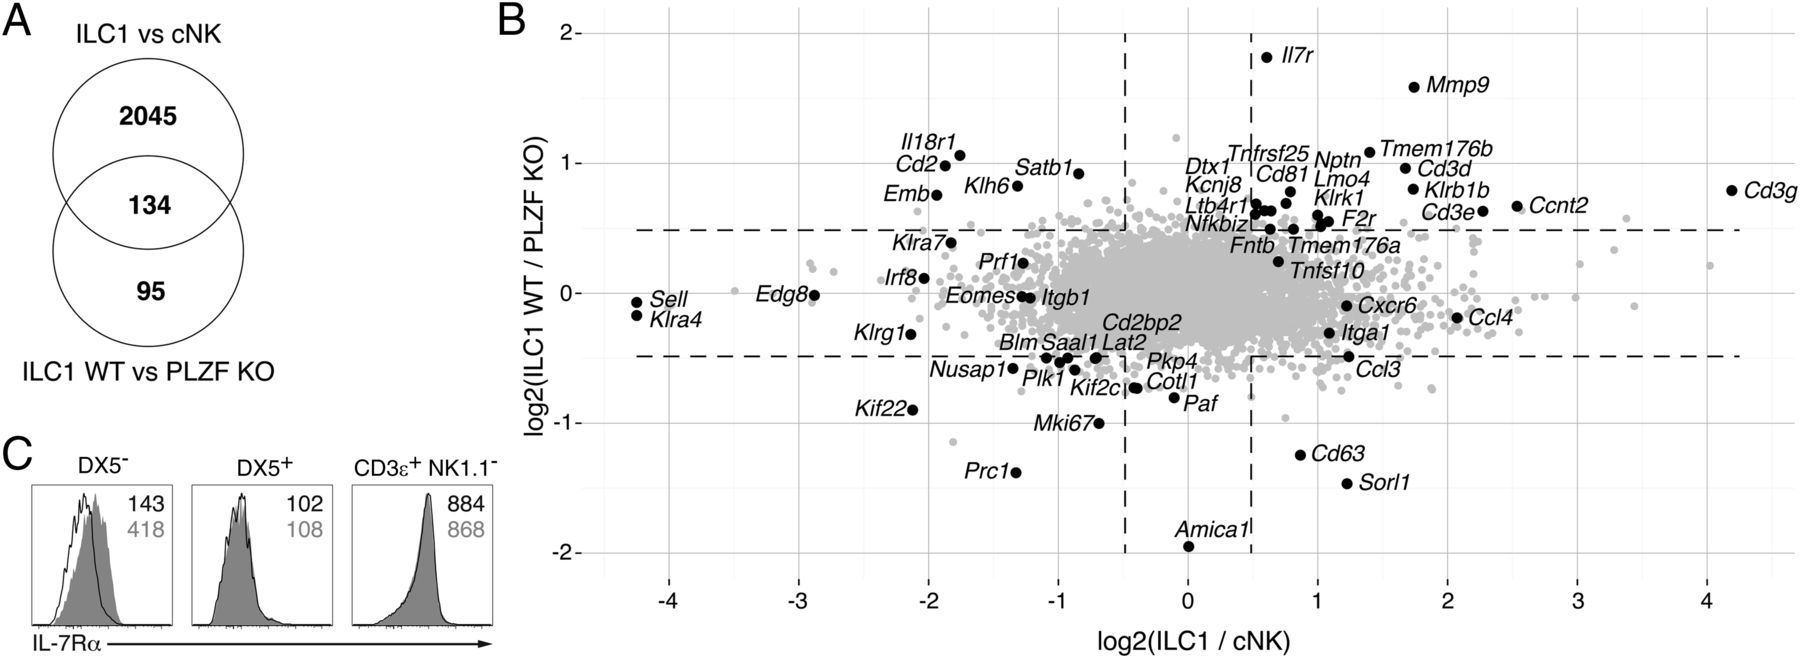
\includegraphics[width=\textwidth]{figures/chapter2/F4}
\end{center}
	\caption{Most PLZF-dependent genes in ILC1s are also differentially expressed between ILC1s and cNKs.} 
	 Shown is a comparison of changes in gene expression due to PLZF deficiency in ILC1s (ILC1 WT/PLZF KO) and changes in gene expression between ILC1s versus cNKs (ILC1/cNK). (A) Venn diagram. The P value for 134/229 PLZF-dependent genes to be part of the 2,179 genes differentially expressed between ILC1s and cNKs is $2.7 \times 10^{−93}$ by hypergeometric test. (B) Scatter plot. Dotted lines delineate the 1.4-fold change threshold. Select immune genes are highlighted. (C) FACS analysis of IL7R$\alpha$ expression by liver ILC1s (DX5\UM) and cNKs (DX5\UP) from PLZF\U{--/--} (open) and WT littermates (filled gray), with T cells as positive controls (\CDte\UP NK1.1\UM). Mean fluorescence intensity (MFI) is indicated in black for PLZF\U{--/--} and gray for WT. Representative of 4 WT and 4 PLZF\U{--/--} littermates examined in two separate experiments.
	\label{fig:chap2_F4}
\end{figure}

\section{DISCUSSION}

This study uses PLZF reporting and fate-mapping to identify developmental intermediates in the ILC1 lineage pathway and to define their relationship with previously proposed stages of cNK development. Whereas the history of expression of PLZF and \ab{} clearly distinguished ILC1 from cNK precursors, the subsequent developmental intermediates appeared to be intermixed within the rNKP and iNK stages, which were previously assigned solely to cNKs. The earlier, pre-NKP stage appeared to be an even more complex mixture of PLZF-expressing ILCPs, which can give rise to ILC1s, ILC2s, and ILC3s, and of PLZF-negative cNK precursors. In contrast, the so-called “pre–pro-NK” cells, previously shown to generate NK1.1\UP{} cells in single-cell culture with OP9 and IL-15, include a majority of immature ILC2s, suggesting that these cells might exhibit a degree of plasticity in forced cytokine environments, as reported recently for more mature ILC lineages \cite{klose2013,huang2015}.

The earliest committed precursor to the cNK lineage has not been physically identified yet. Although the PLZF\UM \ab\UM{} fraction of pre-NKPs is likely associated with the cNK lineage, recent studies using transfer experiments into \Ragrg hosts suggested that an earlier cNK precursor might be found at a post-CLP stage defined by a Lin\UM IL7R$\alpha$\UP \ab\U{high} Id2\U{low} PLZF\U{low/neg} profile \cite{klose2014,yu2014}. These cells might then rapidly down-regulate \ab{} to become pre-NKPs in the cNK pathway. Thus, whereas ILC1s and cNKs both require NFIL3 and Tox at an early phase of their development, the divergence between these lineages is associated with the differential regulation of \ab{} and PLZF, and possibly other factors such as Id2 and Gata3, which are also expressed at very high levels in ILCPs \cite{constantinides2014}. The divergence between these lineages and the parallel stages of their development are depicted in Fig. \ref{fig:chap2_S2}.

Our study demonstrates that PLZF accompanies but is not absolutely required for this divergence. Indeed, PLZF has a detectable impact, as demonstrated by the observation that most of the PLZF-dependent genes in ILC1s, including the characteristic Il7r, are also differentially expressed between ILC1s and cNKs. However, this impact is relatively modest compared, for example, with NKT thymocyte development, where PLZF is absolutely essential for the acquisition of the T-helper polarized effector programs, which closely mirrors the trifurcation of ILCPs into ILC1, ILC2, and ILC3 lineages. This surprising difference may reflect the presence of redundant gene(s) in ILCPs or, alternatively, may suggest that PLZF-deficient ILC1s are expanded from a fraction of precursors that overcome defective survival signals, for example through the IL7 receptor, but are otherwise relatively normal. Future studies of the redefined early stages of cNK and ILC development should help unravel the transcriptional events controlling these innate lymphoid lineages and elucidate the molecular basis of their divergence.

\section{METHODS}

\textit{Mice}. C57BL/6J (stock no. 000664), B6.SJL-\textit{Ptprc}\U{a} \textit{Pepc}\U{b}/BoyJ (CD45.1; stock no. 002014), and B6.129 × 1-Gt(ROSA)26Sor\U{tm1(EYFP)Cos}/J (stock no. 006148) mice were obtained from The Jackson Laboratory, whereas B6.Rag2\U{tm1Fwa} II2rg\U{tm1Wjl} (\Ragrg, stock no. 4111) mice were obtained from Taconic. The PLZF\U{GFPcre} strain has been described (15). PLZF\U{--/--} mice were a gift from P. P. Pandolfi, Beth Israel Deaconess Medical Center, Boston, and were backcrossed to C57BL/6J for at least nine generations. Unless noted otherwise, animals were 4–10 wk of age when analyzed and were compared with littermate controls obtained from crosses between heterozygous breeders. For fetal experiments, the morning a vaginal plug was observed was considered E0. Mice were housed in a specific pathogen-free environment at the University of Chicago, and experiments were performed in accordance with the guidelines of the Institutional Animal Care and Use Committee.
\\
\textit{Preparation of Cell Suspensions}. Spleen and liver were mechanically dissociated through 70-$\mu$m filters, and bone marrow was isolated by gently crushing femurs and tibias before filtration. Following dissociation, each liver was centrifuged at 400 × g for 5 min, resuspended in 5 mL of 40\% (vol/vol) Percoll (Sigma-Aldrich), and then centrifuged at 800 × g for 10 min. The supernatant was aspirated and the cell pellet was resuspended in HBSS (Gibco) containing 0.25\% BSA (Sigma-Aldrich) and 0.65 mg/L sodium azide (Sigma-Aldrich).
Flow Cytometry. Cell suspensions were incubated with purified anti-CD16/32 (clone 93) for 10 min on ice to block Fc receptors. Fluorochrome- or biotin-labeled monoclonal antibodies (clones denoted in parentheses) against \ab{} (DATK32), B220 (RA3-6B2), \CDte{} (145-2C11), CD4 (RM4-5 or GK1.5), CD8$\alpha$ (53-6.7), CD11b (M1/70), CD11c (N418), CD19 (6D5), CD25 (PC61), CD27 (LG.7F9), CD45.1 (A20), CD45.2 (104), CD49a (HM$\alpha$1), CD122 (5H4 or TM-$\beta$1), CD160 (7H1), CD244 (2B4), cKit (2B8), DX5 (DX5), Eomes (Dan11mag) Flt3 (A2F10), Gr-1 (RB6-8C5), ICOS (C398.4A), \IFNg (XMG1.2), IL-7R$\alpha$ (A7R34), Ly-6D (49-H4), NK1.1 (PK136), NKp46 (29A1.4), Sca-1 (D7), T1/ST2 (D1H9), TCR$\beta$ (H57-597), Ter-119 (TER-119), Thy1.2 (53-2.1) and TRAIL (N2B2) were purchased from BD Biosciences, BioLegend, eBioscience, or R\& D Systems. To exclude dead cells, 4',6-diamidino-2-phenylindole (DAPI; Molecular Probes) was added to all live samples. For intracellular staining, cells were fixed with 4\% paraformaldehyde and permeabilized by using the Foxp3 Transcription Factor Staining Buffer Set (eBioscience). Cells were run on an LSRII (BD Biosciences) or sorted by using a FACS Aria II (BD Biosciences) and analyzed by using FlowJo software (Tree Star). Collected events were gated on DAPI− lymphocytes and doublets were excluded.
Unless specified otherwise, CLPs were gated Lin\UM Ly6D\UM CD244\UP CD27\UP IL-7R$\alpha$\UP Flt3\UP CD122\UM{} (19), pre-NKP were gated Lin\UM Ly6D\UM CD244\UP CD27\UP IL-7R$\alpha$\UP Flt3\UM CD122\U{low/neg} (19), rNKP were gated Lin\UM Ly6D\UM CD244\UP CD27\UP IL-7R$\alpha$\UP Flt3\UM CD122\U{high} (19), pre–pro-NK were gated Lin\UM Sca-1\UP cKit\U{low} IL-7R$\alpha$\UP Flt3\UM{} (20), bone marrow DX5\UM{} cells were gated Lin\UM CD122\UP NK1.1\UP NKp46\UP DX5\UM{} (14), bone marrow DX5\UP cells were gated Lin\UM CD122\UP NK1.1\UP NKp46\UP DX5\UP, liver DX5\UP cells were gated \CDte\UM TCR$\beta$\UM NK1.1\UP DX5\UP CD49a\UM, and liver DX5\UM{} cells were gated \CDte\UM TCR$\beta$\UM NK1.1\UP DX5\UM CD49a\UP. Lineage mixtures for pre-NKPs, rNKPs, and CLPs included antibodies against \CDte, CD11b, CD19, and NK1.1; for pre–pro-NK: \CDte, CD8$\alpha$, CD11b, CD19, Gr-1, and Ter119; for bone marrow NK1.1\UP subsets: \CDte, CD4, CD8$\alpha$, CD19, and Ter119.
\\
\textit{Bone Marrow Chimeras}. To generate YFP\UM chimeras, $5–10 \times 10^3$ LSK cells were sorted from the bone marrow of PLZF\U{GFPcre+/--} ROSA-YFP mice and injected retroorbitally into lethally irradiated (1,000 rads) CD45.1 recipients. Chimeras were analyzed 5–7 wk after reconstitution, gating on CD45.2\UP cells to exclude residual host cells.
\\
\textit{Isolation and Adoptive Transfer of Bone Marrow CLPs and NK1.1\UP{} Subsets}. For the isolation of CLPs from CD45.1 bone marrow, lineage\UP cells were first depleted by using an autoMACS (Miltenyi Biotec) after staining with biotin-conjugated antibodies against B220, \CDte, CD4, CD8$\alpha$, CD11b, CD11c, CD19, Gr-1, NK1.1, TCR$\beta$, and Ter119, followed by incubation with SAv microbeads (Miltenyi Biotec). CLPs were then sorted as DAPI\UM Lin\UM IL-7R$\alpha$\UP cKit\U{int} Sca-1\U{int} Flt3\U{high} to greater than 95\% purity by using a FACS Aria II (BD Biosciences). For the isolation of YFP\UP NK1.1\UP DX5\UM{} cells, bone marrow from YFP\UM{} chimeras (described above) was stained with APC-conjugated anti-NK1.1 antibody, bound to anti-APC microbeads (Miltenyi Biotec), subjected to double-column enrichment, and sorted as DAPI\UM Lin\UM CD122\UP NK1.1\UP NKp46\UP DX5\UM YFP\UP to greater than 95\% purity. For the isolation of NK1.1\UP DX5\UM{} cells, CD45.1 bone marrow was stained with APC-conjugated anti-NK1.1 antibody, bound to anti-APC microbeads, subjected to double-column enrichment, and sorted as DAPI\UM Lin\UM CD122\UP NK1.1\UP NKp46\UP DX5\UM to greater than 95\% purity. For the NK1.1\UP subsets, the lineage mixture antibodies used were as follows: \CDte, CD4, CD8$\alpha$, CD19, and Ter119.
Following isolation, 1,500 YFP\UP NK1.1\UP DX5\UM{} cells mixed with 750 CD45.1-congenic CLPs, or 1,500 CD45.1 NK1.1\UP DX5\UM{} cells alone were injected retroorbitally into sublethally irradiated (400 rads) 6- to 10-wk-old CD45.2 \Ragrg mice. Recipient mice were analyzed 3–4 wk after transfer.
\\
\textit{Isolation and in Vitro Stimulation of NK1.1\UP DX5\UM{} Cells}. Following enrichment using FITC-NK1.1 and anti-FITC microbeads (Miltenyi Biotec), NK1.1\UP DX5\UM cells were sorted as DAPI\UM Lin\UM NK1.1\UP NKp46\UP DX5\UM from the bone marrow or DAPI\UM \CDte\UM TCR$\beta$\UM NK1.1\UP NKp46\UP DX5\UM from the liver of WT mice ($>$95\% purity). For the bone marrow cells, the lineage mixture antibodies used were the following: \CDte, CD4, CD8$\alpha$, CD19, TCR$\beta$, and Ter119. Up to 10,000 sorted cells were resuspended in 500 $mu$L of RPMI medium 1640 (Cellgro) containing 10\% FCS (Biowest) and 1× GolgiStop (BD). Samples were stimulated with phorbol 12-myristate 13-acetate (PMA; 20 ng/mL) and ionomycin (5 $\mu$g/mL) for 4 h at 37 °C. Following the stimulation, samples were fixed and permeabilized by using the Cytofix/Cytoperm kit (BD).
\\
\textit{Microarray Analysis}. Liver lymphocytes from pools of PLZF\U{+/+} or PLZF\U{--/--} mice were sorted into ILC1s (\CDte\UM NK1.1\UP CD49a\UP DX5\UM) and cNKs (\CDte\UM NK1.1\UP CD49a\UM DX5\UP) and stored in TRIzol (Life Technologies). RNA was isolated by using the RNeasy mini kit (Qiagen), processed, and annealed to the mouse WG-6 array (Illumina). Illumina MouseWG-6 v2.0 Expression BeadChip data were quality-checked by using the lumi package \cite{du2008} and quality control metrics in the R/Bioconductor statistical software package (v3.0.0). Data were background corrected and normalized by variance-stabilizing transformation \cite{lin2008} followed by quantile normalization. Data were log2 transformed and fit to linear models by using the limma package \cite{smyth2005} for fold change comparison between groups. A fold-change cutoff of 1.4 was used to distinguish differentially expressed genes. Microarray data has been deposited with the National Center for Biotechnology Information Gene Expression Omnibus repository under the accession number GSE65898.
\\
\textit{Statistical Analysis}. Two-tailed Student’s t test was performed by using Prism (GraphPad Software) to determine whether data differed from the expected value. *$P < 0.05$.

\subsubsection{Acknowledgments}
This work was supported by NIH Grants R01 AI108643, AI038339, and HL118092 (to A.B.) and University of Chicago Digestive Diseases Research Core Center Grant P30 DK42086.

%% FIGURE NUMBERING %%
\renewcommand\thefigure{\thechapter.S\arabic{figure}} 

\newpage
\section{SUPPORTING INFORMATION}
\setcounter{figure}{0}

%% Chapter 2 Figure S1 pre-proNK and ILC2s %%
\begin{figure}[h]
\begin{center}
	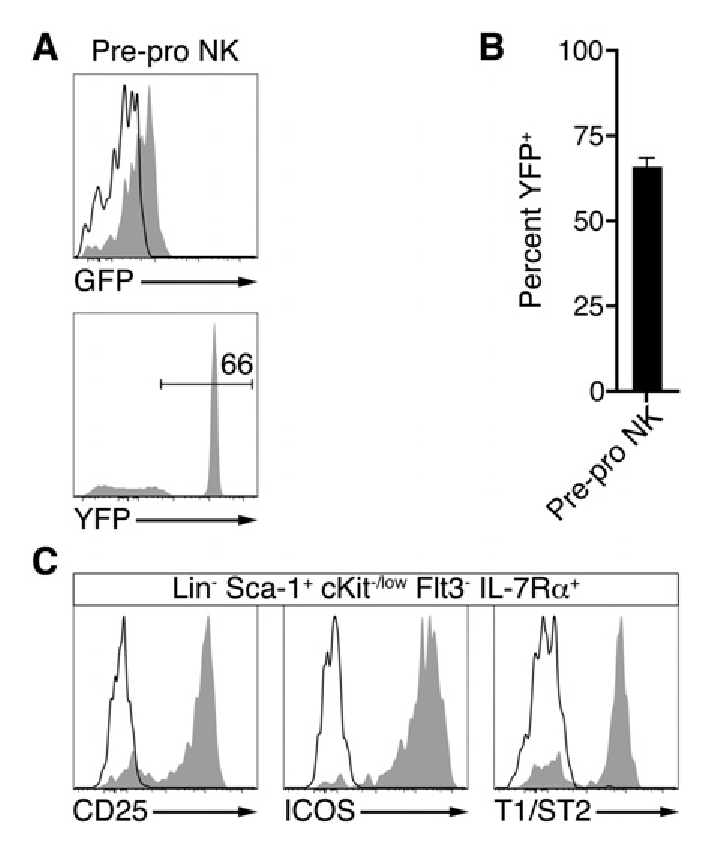
\includegraphics[width=0.4\textwidth]{figures/chapter2/S1}
\end{center}
	\caption{Pre-pro-NKs contain a majority of immature ILC2s.} 
	 (A, Top) Expression of GFP (reporting PLZF) by the pre-pro-NK population (Lin\UM Sca-1\UP cKit\U{--/low} Flt3\UM IL-7R$\alpha$\UP) from PLZF\U{GFPcre+/+} (filled gray) and WT (open) mice. (Bottom) YFP expression (reporting fate-mapping by PLZF) in YFP-negative radiation chimeras. (B) Summary of results (mean $\pm$ SEM) shown in A. (C) FACS analysis of pre-pro-NK cells, stained for indicated markers (filled gray) or with isotype controls (open). Data representative of at least three mice analyzed in two or more independent experiments.
	\label{fig:chap2_S1}
\end{figure}

%% Chapter 2 Figure S2 Divergence diagram %%
\begin{figure}[p]
\begin{center}
	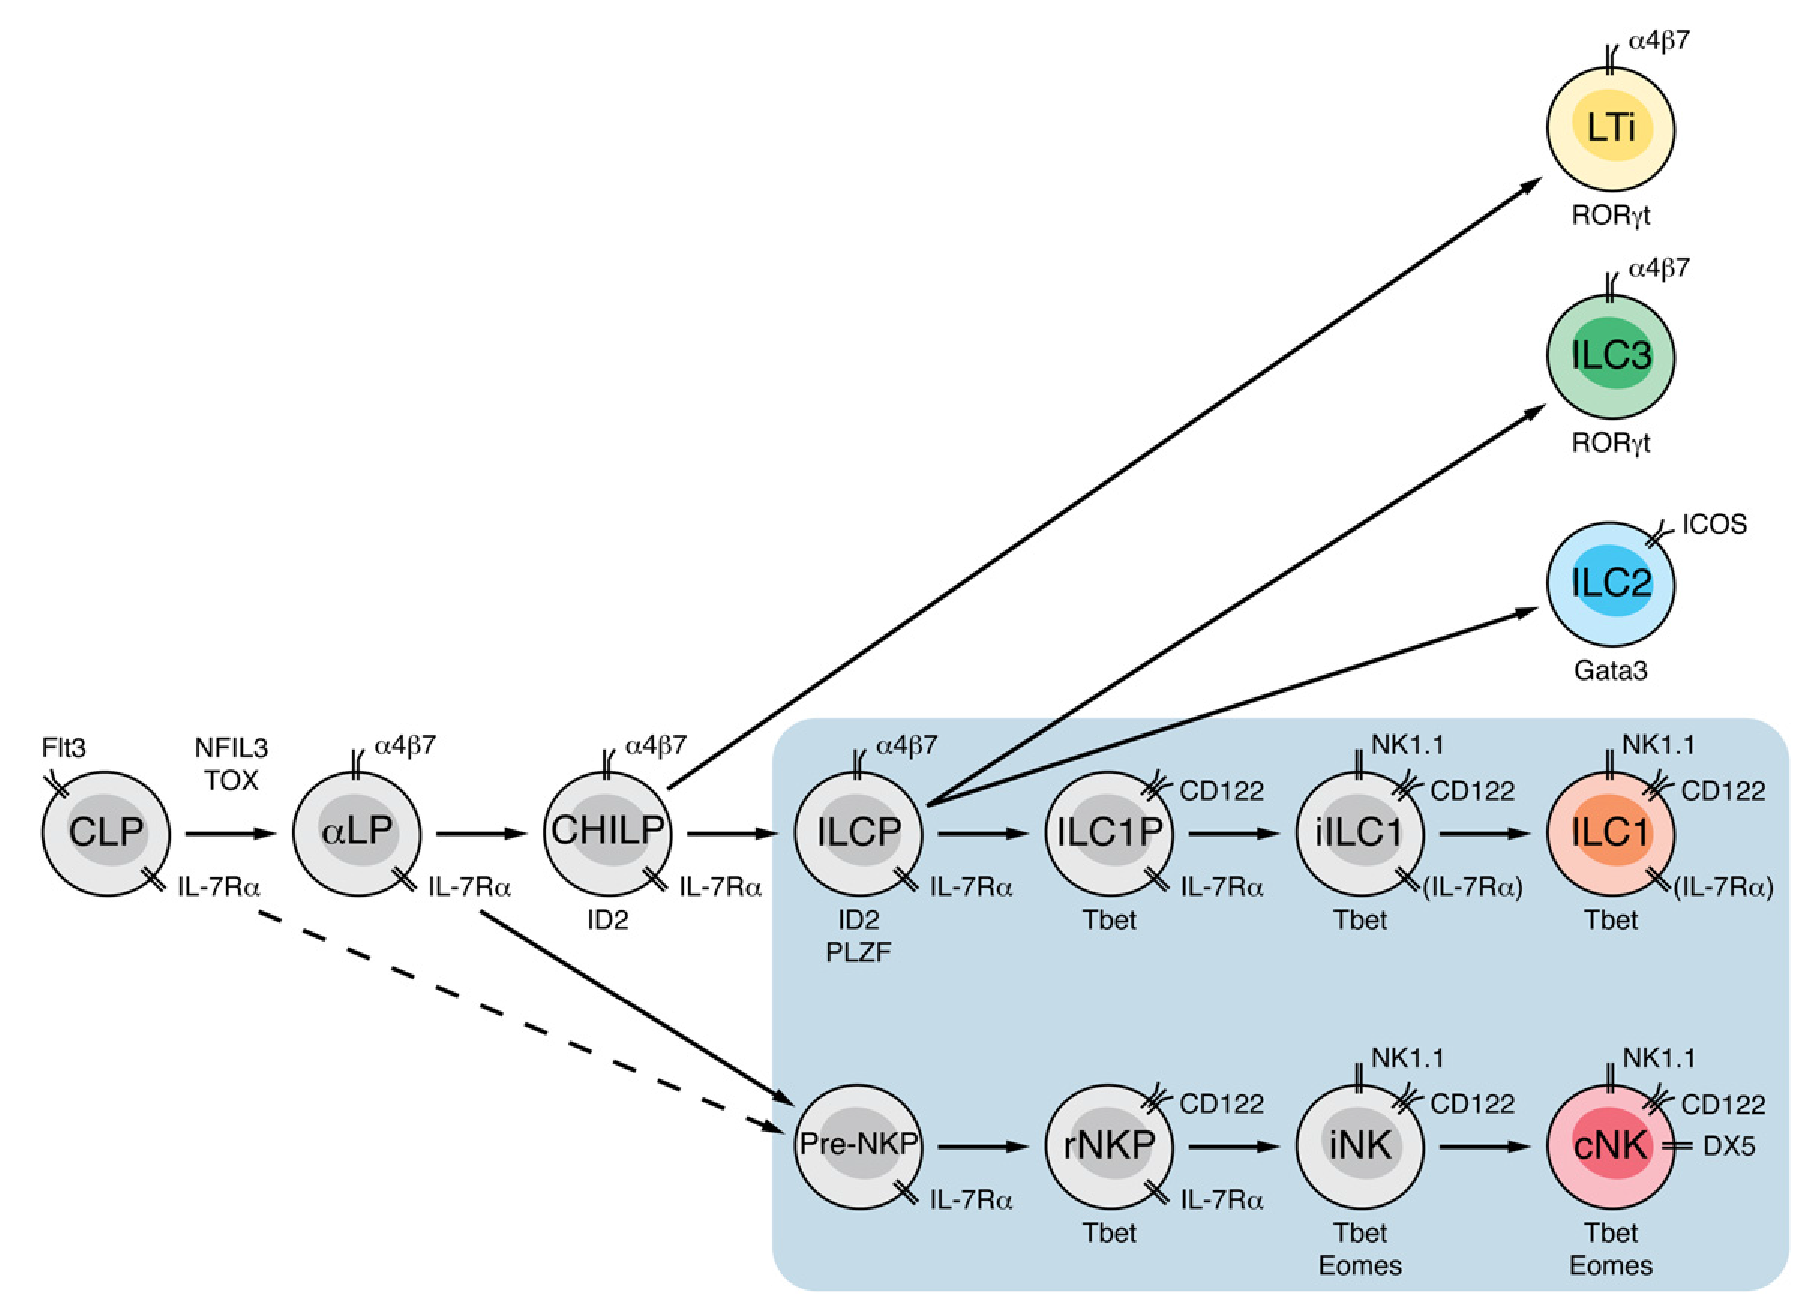
\includegraphics[width=\textwidth]{figures/chapter2/S2}
\end{center}
	\caption{Divergence and parallels in the development of ILC1s and cNKs.} 
	 The diagram highlights, within the shaded rectangle, the parallel progression sequence of ILC1 and cNK progenitors, with ILCP, ILC1P, and iILC1 previously included in, and now distinguished from, pre-NKP, rNKP, and iNK, respectively. The abbreviated names of developmental intermediates include CLP (common lymphoid precursor), \aLP (\ab\UP lymphoid precursor), CHILP (common helper innate lymphocyte precursor), ILCP (innate lymphoid cell precursor), ILC1P (ILC1 precursor), iILC1 (immature ILC1), pre-NKP (pre-NK precursor), rNKP (refined NKP), iNK (immature NK), and mNK (mature NK).
	\label{fig:chap2_S2}
\end{figure}

%% REVERT FIGURE NUMBERING %%
\renewcommand\thefigure{\thechapter.\arabic{figure}} 

%%% END CHAPTER 2 MICROARRAY %%%

